\documentclass[licencjacka,openright]{pracamgr}
\usepackage{latexsym}
\usepackage[MeX]{polski}
\usepackage[utf8]{inputenc}
\usepackage{graphicx}
%\usepackage{afterpage}
\usepackage{rotating}
%\usepackage{subfigure}%
\usepackage{polski}
\usepackage{natbib}
\usepackage{indentfirst}
\usepackage{graphicx}
\usepackage{url}
\usepackage{float}
\usepackage{amsmath}
\usepackage{antpolt}
\usepackage[T1]{fontenc}
\usepackage[draft]{todonotes}
\usepackage{hyperref}
\usepackage{booktabs}
\usepackage{chngcntr}
\usepackage[font={small,it}]{caption}
\usepackage[section]{placeins}


\author{ Karol Auguštin }
\nralbumu{ 249476 }
\title{ Filtry przestrzenne w detekcji potencjału P300 }
\tytulang{ Spatial filters in detection of P300 evoked potential }
\kierunek{Zastosowania fizyki w biologii i medycynie}
\opiekun{dr hab. Jarosława Żygierewicza \\ Zakład Fizyki Biomedycznej \\ Instytut Fizyki Doświadczalnej \\ Wydział Fizyki \\ Uniwersytet Warszawski}
\dziedzina{13.2 Fizyka}
\specjalnosc{Neuroinformatyka}
\date{Warszawa, Wrzesień 2013}
\keywords{P300, filtry przestrzenne, interfejsy mózg -- komputer, CSP} 

%\bibliographystyle{elsart-harv}
%\bibliographystyle{unsrt}
\bibliographystyle{apalike}

\begin{document}
\let\cleardoublepage\clearpage
\maketitle
\begin{abstract}
\par W pracy zaprezentowano i przetestowano doświadczalnie zastosowanie filtrów przestrzennych w detekcji wystąpienia potencjału P300 w urządzeniach BCI. Uzyskane rezultaty potwierdzają skuteczność stosowania tych filtrów w algorytmach detekcji potencjałów wywołanych w czasie rzeczywistym.
\end{abstract}
\tableofcontents


\chapter{Wstęp}
\section{Potencjały wywołane}
\label{potencjaly}
Potencjały wywołane (ERP) są to zmiany w potencjale elektrycznym mózgu rejestrowane najczęściej na powierzchni czaszki. Występują one w odpowiedzi na bodziec podawany pacjentowi. W niniejszej pracy analizowany będzie przebieg potencjału P300, który jest potencjałem endrogennym występującym po zauważeniu przez pacjenta bodźca oczekiwanego pośród innych, nieoczekiwanych, bodźców. W pracy potencjał P300 wywoływano wzrokowo, ale można go również wywoływać słuchowo oraz czuciowo. 
Z uwagi na niską amplitudę ERP występowanie ich można zauważyć uśredniając wiele przebiegów (realizacji) minimalizując składową sygnału pochodzącą od procesów nie związanych z badanym potencjałem.
Badany potencjał P300 występuje około 300ms po podaniu bodźca i charakteryzuje się przebiegiem w niskich częstotliwościach. 

\section{Diagnostyka medyczna}
Istnieje wiele udokumentowanych zastosowań detekcji potencjału P300 w~diagnostyce medycznej chorób układu nerwowego, zaburzeń psychicznych, a~także uszkodzeń mózgu w~wyniku urazów \citep{zgorzalewicz2000}. Opierają się one głównie na analizie wielu cech rejestrowanego potencjału takich jak: latencja względem bodźca, kształt, oraz miejsce występowania na powierzchni czaszki. Praktycznie we~wszystkich przypadkach opisanych w~literaturze sposób badania jest identyczny, jeśli porównywany jest od strony analizy sygnału. Pacjentowi podawany jest wielokrotnie bodziec standardowy (ang. target), przeplatany z bodźcem celowym (ang. non-target), mającym wygenerować u pacjenta potencjał P300. Następnie przeprowadzane jest uśrednianie wystąpień bodźca celowego dla każdej z~elektrod i~analiza takiego wyniku wykonywana przez lekarza. 
W związku z~tym, że~najistotniejszym elementem badania diagnostycznego jest amplituda oraz czas wystąpienia reakcji (latencja), jak również umiejscowienie jej na~powierzchni czaszki \citep{chudzik2004} jedynymi powszechnie stosowanymi metodami analizy sygnałów są~filtrowanie pasmowe i~uśrednianie, natomiast nie jest praktykowane użycie filtrów przestrzennych, czy innych metod mających na celu lepsze uwidocznienie potencjału.

\section{Interfejsy mózg -- komputer}
Najbardziej obiecującym zastosowaniem zautomatyzowanej analizy sygnału EEG są~obecnie interfejsy mózg-komputer (brain-computer interface -- BCI) mające na~celu umożliwienie komunikacji użytkownika z~komputerem bez użycia mięśni a jedynie lub głównie poprzez analizę sygnału EEG zbieranego z powierzchni czaszki użytkownika. Aby umożliwić wykorzystanie potencjału P300 w~takim zastosowaniu potrzebny jest złożony z~wielu elementów aparat matematyczno -- informatyczny, za~pomocą którego w~zautomatyzowany sposób można by rejestrować wystąpienie w pojedynczej lub niewielkiej ilości realizacji potencjałów P300 w~sposób nie~wymagający udziału przeszkolonej osoby. Jako, że~w~takiej sytuacji istotny jest nie kształt czy opóźnienie załamka P300, a~samo jego wystąpienie w~reakcji na~określony bodziec dostępne są~wszystkie metody cyfrowej analizy sygnałów, o~ile okażą się~skuteczne.

\subsection{Dostęp do informacji}
Od lat osiemdziesiątych mamy do~czynienia z~dynamicznym rozwojem informatyzacji społeczeństwa, nie~tylko w~warstwie możliwości technicznych, ale~przede wszystkim w~rozumieniu społecznym. Przez ostatnie trzydzieści lat stopień zastosowania komputerów i~urządzeń elektronicznych przez społeczeństwo wzrósł, a~co~ważniejsze wzrost ten nadal występuje w~olbrzymim tempie. Unowocześnianie i~ułatwianie ludziom dostępu do~komputerów i~możliwości jakie ten dostęp umożliwia jest kluczowym zadanie producentów i~projektantów wszystkich firm produkujących urządzenia elektroniczne przeznaczone dla masowego odbiorcy. Sposób komunikacji użytkowników z~komputerem ewoluował na przestrzeni lat. Od klawiatury podłączonej do~terminala tekstowego w~latach osiemdziesiątych przez wprowadzenie na~rynek myszki i~interfejsu graficznego przez firmę Apple Computers Inc. w~1984 roku, aż~do~obecnie znanych i~coraz szerzej stosowanych ekranów dotykowych. Historia komunikacji człowieka z urządzeniami elektronicznymi pokazuje jak istotny dla współczesnego świata jest sposób dostępu człowieka do możliwości jakie dają współczesne komputery.

Rozwój urządzeń umożliwiających komunikację ludzi z~komputerami opiera się na~stosowaniu technologii eliminujących nienaturalnych i~zbędnych urządzeń pośredniczących w tejże komunikacji. Najpierw ograniczono rolę klawiatury, na~rzecz dużo prostszej i~bardziej naturalnej myszki, żeby w końcu i~z~niej zrezygnować na rzecz ekranu obsługiwanego w naturalny dla człowieka sposób -- palcami. Kolejnym krokiem w~tej ewolucji jest wyeliminowanie konieczności używania jakiegokolwiek urządzenia obsługiwanego za pomocą mięśni na rzecz bezpośredniego połączenia komputera z~mózgiem użytkownika.

\subsection{Pomoc osobom niepełnosprawnym}
Kolejnym aspektem zastosowania systemów BCI w~postaci, w~jakiej istnieją one dzisiaj jest pomoc osobom niepełnosprawnym, w~szczególności sparaliżowanym, pozbawionym możliwości kontaktu ze~światem zewnętrznym za pośrednictwem mięśni. Urządzenia BCI Appliance tworzone i~rozwijane na~wydziale Fizyki Uniwersytetu Warszawskiego już dzisiaj dają taką możliwość \citep{obci}.
Ponadto na świecie rozwijanych jest wiele projektów oprogramowania BCI takich jak OpenVibe~\citep{renard2010}, Pyff \citep{venthur2008} czy BCI2000 \citep{schalk2004}.

Opierając się na znanych mechanizmach działania mózgu umożliwiają wprowadzanie informacji do komputera jedynie za pomocą analizy sygnału EEG związanego z koncentracją uwagi na określonych bodźcach. Jednym z paradygmatów, na którym opiera się ten system jest właśnie rejestracja i~analiza potencjału P300.

\section{Cel pracy}
Celem pracy jest zbadanie oraz zaprezentowanie jak~zastosowanie filtrów przestrzennych wpływa na~możliwość wykrywania występowania potencjału P300. Opracowanie
algorytmu i jego sprawdzenie w zastosowaniu występującym w maszynach BCI. Przyczynia się to do konstrukcji lepszych BCI opartych o paradygmat P300.

\chapter{Metodologia}
Potencjał P300 występujący w~sygnale EEG w~reakcji na~oczekiwany przez pacjenta bodziec ma złożoną charakterystykę, czyniąc go trudnym do automatycznej detekcji. Podstawowym problemem jest mała amplituda zjawiska na tle innych aktywności mózgu widocznych w sygnale EEG oraz duża zmienność osobnicza i zależność od wielu czynników takich jak wiek i płeć osoby badanej, czas od ostatniego posiłku, rodzaj oraz trudność w zauważeniu bodźca oraz motywacja~\citep{chudzik2004}.
Jedyną metodą uzyskania widocznego gołym okiem potencjału bez stosowania skomplikowanego aparatu matematycznego jest uśrednienie wielu realizacji eksperymentu. W takim przypadku aktywność mózgu nie związana z~występowaniem interesującego nas zjawiska jest modelowana jako szum nieskorelowany o~średniej zero, zatem ulega uśrednieniu do zera, a~interesująca nas, powtarzająca się dla każdej realizacji aktywność staje się widoczna. Takie podejście, poprawne w przypadku diagnostyki medycznej, niestety nie jest możliwe do~zastosowania w~systemach BCI, gdyż obniżyłoby skuteczność takiego systemu wymuszając na użytkowniku wielokrotne powtarzanie tej samej decyzji. Niski stosunek sygnału do szumu dla potencjału P300 bardzo utrudnia jego wykrycie przy użyciu jednej realizacji. Aby zminimalizować liczbę niezbędnych powtórzeń występowania bodźca zaczęto stosować różnego rodzaju metody mające na celu wyeksponowanie go z szumu pozostałych aktywności mózgu, nie związanych z bodźcem podawanym pacjentowi.

Do najprostszych metod stosowanych w pierwszej kolejności należą przede wszystkim filtrowanie dolnoprzepustowe.

Bardziej zaawansowanymi metodami jest zaprojektowanie odpowiednich filtrów przestrzennych, mających na celu poprawę stosunku sygnału do szumu korzystając z~różnicy w rozkładzie przestrzennym szumu i~interesującej nas aktywności. Przykłady takich filtrów zostaną przedstawione w~kolejnych paragrafach.

\section{Filtry przestrzenne}
Filtry przestrzenne poprawiają stosunek sygnału do szumu wykorzystując różny rozkład przestrzenny składowej będącej sygnałem i~składowej będącej szumem, czyli sygnałem nie~zawierającym składowych istotnych z punktu widzenia badanego zagadnienia.
Filltr przestrzenny może być zrealizowany w postaci macierzy $M$ takiej,~że: 
Y = M*X
gdzie: $X$ oznacza sygnał mierzony, natomiast $Y$ sygnał filtrowany.

\subsection{Filtr tożsamościowy}
Aby zaobserwować efekty uzyskane za~pomocą różnych filtrów przestrzennych przedstawię dane zarejestrowane podczas eksperymentów bez użycia żadnego z~nich. Macierz przejścia dla takich danych jest macierzą, która na diagonali ma~wartości~1~oraz~0~w~pozostałych polach.
Dla trzech kanałów taka macierz ma~postać:
\[
M =
\begin{bmatrix}
  $1$ & $0$ & $0$ \\
  $0$ & $1$ & $0$ \\
  $0$ & $0$ & $1$ 
\end{bmatrix}
\]

\subsection{Transformata Hjorta}
Transformacja Hjortha \citep{hjorth1975} jest numerycznym przybliżeniem transformaty Laplace'a czyli drugiej pochodnej przestrzennej. Uzyskuje się ją poprzez odjęcie od każdego kanału średniej z kanałów go otaczających. Ma on na celu eliminację składowej wspólnej dla transformowanych kanałów, czyli pochodzącej od~źródeł odległych. Sygnał pozostający w~każdym kanale po zastosowaniu takiego filtra powinien odwzorowywać aktywność EEG zachodzącą bezpośrednio w~miejscu umieszczenia elektrody, eliminując czasem mocniejszą aktywność z~innych obszarów czaszki.
Macierz przejścia w~przypadku zastosowania takiego filtra jest ściśle związana z~lokalizacją elektrod na głowie pacjenta.
Transformacja ta ma postać przykładowo w~systemie EEG 10-20 dla elektrody $Cz$ ma~on~postać:
\begin{equation}
V'_{Cz} = V_{Cz} - 1/4(V_{Fz}+V_{C4}+V_{Pz}+V_{C4})
\end{equation}

\subsection{Wspólny wzorzec przestrzenny}
Wspólny wzorzec przestrzenny (ang. Common Spatial Patterns, CSP) \citep{koles1990} jest dyskryminacyjnym algorytmem pozyskującym przestrzenny filtr $W$ z~danych $X$, tak że różnica wariancji filtrowanego sygnału \mbox{$X_{CSP} = X \cdot W$} dla dwóch klas jest maksymalna w pewnym kanale $X_{CSP}$. Osiągane jest to poprzez jednoczesną diagonalizację macierzy kowariancji \citep{samsek2012}:
\begin{equation}
\Sigma _2 W = (\Sigma _1 + \Sigma _2 )W \Delta
\end{equation}
gdzie $\Sigma_1$ i $\Sigma_2$ są kowariancjami macierzy sygnałów z~klas~1~oraz~2. Każda kolumna $W$ jest filtrem przestrzennym $w_i$ odpowiadającym wartości własnej $\delta _i$ w~macierzy $\Delta$, wartości $i = 1,2,3 \ldots N_c$ odpowiadają numerom kanałów sygnału oryginalnego.

\section{Miara jakości}
\label{miara}
Jakość wstępnej analizy sygnałów jest tym lepsza im~zbiór cech wydobytych z~sygnału zarejestrowanego jako target jest bardziej różny od cech sygnału non-target będącego szumem z~punktu widzenia analizowanego zagadnienia.

Zgodnie z powszechnie używanym modelem potencjału wywołanego (sygnał deterministyczny + szum niezależny) proponowaną cechą różnicującą jest maksymalna wartość funkcji korelacji punkcie zero pomiędzy średnią z sygnałów target uzyskanych podczas sesji kalibracyjnej oraz sygnałem poddawanym analizie.

Możliwa do osiągnięcia jakość klasyfikacji nieznanych próbek jako elementów różnych klas jest tym większa im większa jest separacja rozkładów cech dla tych klas. Jako miarę separacji rozkładów w przestrzeni wielowymiarowej można zastosować odległość Mahalanobisa. Wyraża się ona wzorem:

\begin{equation}
d_{m}{(x,y)}=\sqrt{(x-y)\Sigma^{-1}(x-y)^T}
\end{equation}
gdzie: $x$, $y$ są wektorami danych porównywanych, a $\Sigma$ macierzą kowariancji.

Dla sytuacji jednowymiarowej odległość ta redukuje się do miary $t$, co ma intuicyjną interpretację mierzenia odległości w jednostkach odchylenia standardowego:
\begin{equation}
t = \frac{x-\mu}{s_x}
\end{equation}
gdzie: $x$ jest wektorem danych, $\mu$ jest średnią z wektora danych, a $S_x$ odchyleniem standardowym danych.

W celu osiągnięcia jak najlepszych rezultatów cechy były obliczane dla dwóch kanałów, w których różnica w uśrednionych przebiegach sygnałów target i non-target była największa.

\section{Oprogramowanie}
Oprogramowanie wykorzystane do wykonania symulacji i obliczeń zostało w całości napisane w języku Python~2{.}7. Do obliczeń numerycznych użyto pakietów NumPy~1{.}7{.}1 oraz SciPy~0{.}12{.}0 natomiast do wykonania wykresów pakiet Matplotlib~1{.}3{.}0.

Całość kodu zamieszczono w repozytorium systemu kontroli wersji Git i udostępniono na licencji GPL v3 pod adresem: \url{http://git.nimitz.pl/p300-csp.git}. Wersja użyta w tej pracy oznaczona została tagiem o nazwie: licencjat-p300 i ID: 9eb1ed41ac3450438d7c561807a6c7d3060c204c oraz podpisanym kluczem PGP: 2048R/18C35B1E.

\chapter{Dane}
Dane do analizy opisanych metod były zbierane podczas sesji kalibracyjnej, w~której osoba badana patrzyła się na jeden z~ośmiu losowo zapalających się kwadratów. Dzięki temu zebrane dane opatrzone są~informacją, czy należą do~grupy target, w~przypadku zapalenia się obserwowanego pola, czy non-target w~pozostałych przypadkach.

W obu przypadkach zastosowano próbkowanie z~częstotliwością 128Hz. Zarejestrowano dane z~22~kanałów rozmieszczonych w~systemie 10-20 za pomocą wzmacniacza TMSi Porti7. Do stymulacji wykorzystano urządzenie BCI Appliance z zainstalowanym oprogramowaniem OpenBCI, do zapisywania sygnału użyto programu Svarog \citep{obci}.

Podczas użytej do obliczeń sesji kalibracyjnej zebrano 64 realizacje sygnału target i 528 realizacji sygnału non-target. Do wszystkich obliczeń został zastosowany wstępny montaż danych względem uśrednionych odprowadzeń usznych A1 oraz A2. Do obliczeń sygnał został pocięty na odcinki od $0{,}2$ sekundy przed bodźcem do $0{,}5$ sekundy po bodźcu. Ostatnim etapem przygotowania sygnału było zastosowanie filtru dolnoprzepustowego Butterwortha drugiego rzędu o częstotliwości odcięcia 25Hz. W celu zasymulowania działania algorytmu w urządzeniu BCI filtrowanie przeprowadzono dla każdego przebiegu oddzielnie już po jego pocięciu na poszczególne realizacje.

Filtr górnoprzepustowy nie był zastosowany po rejestracji sygnału, natomiast maksymalna zarejestrowana częstotliwość przez wykorzystany w eksperymencie wzmacniacz przy częstotliwości próbkowania 128Hz wynosi 38Hz.

Od każdego analizowanego odcinka sygnału została odjęta składowa stała aby sygnał w tym odcinku był rozpięty wokół zera.

\chapter{Wyniki}
\label{wyniki}

\section{Wybór kanałów}
\label{sygnaly}

Pierwszym etapem analizy danych był wybór dwóch kanałów, w których jest najlepiej widoczna różnica pomiędzy przebiegami sygnałów target i non-target dla każdego filtru przestrzennego. 

Na rysunkach \ref{macierz_toz}, \ref{macierz_hjorth}, \ref{macierz_csp} przedstawiono macierze uśrednionych sygnałów target i non-target dla wszystkich zarejestrowanych przebiegów. Dla każdego badanego filtru przestrzennego wybrano dwa kanały w których różnica pomiędzy przebiegami target i non-target jest największa.

\subsection{Filtr tożsamościowy}

Na rysunku \ref{macierz_toz} przedstawiono macierz uśrednionych sygnałów dla przebiegów target (czerwony) i non-target (niebieski). Do dalszej analizy wybrano kanały Fz i Cz. Wszystkie przebiegi target i non-target dla tych kanałów przedstawiono na rysunku \ref{sygnal_toz}.

\begin{figure}
\centering
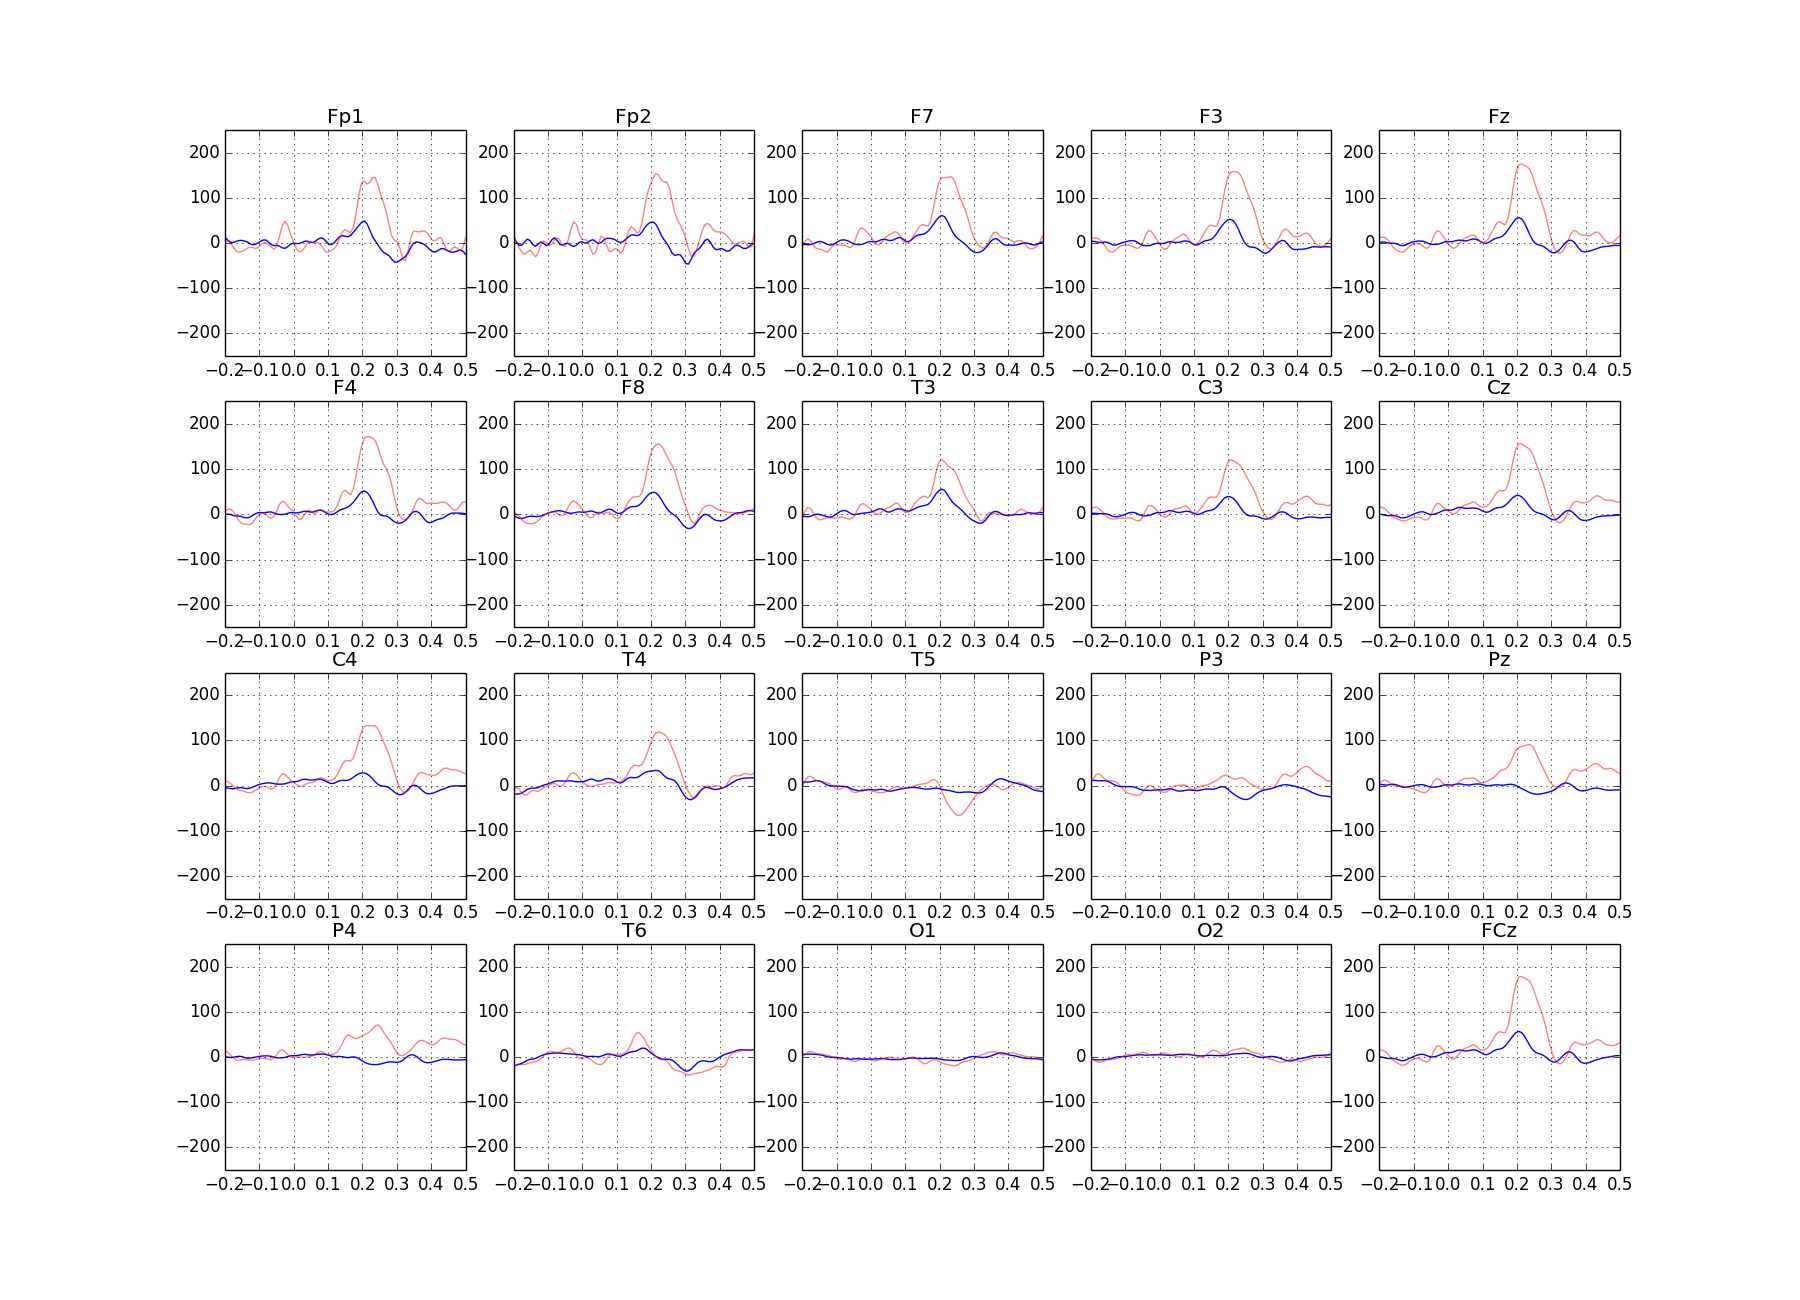
\includegraphics[scale=0.35, trim=10mm 25mm 10mm 25mm, clip=True]{pics/macierz_toz.png}
\caption{Macierz sygnałów uśrednionych target (czerwony) i non-target (niebieski) dla filtru tożsamościowego. Oś odciętych -- potencjał w  $\mu$V, oś rzędnych -- czas w s, zero oznacza wystąpienie bodźca.}
\label{macierz_toz}
\end{figure}

\begin{figure}
\centering
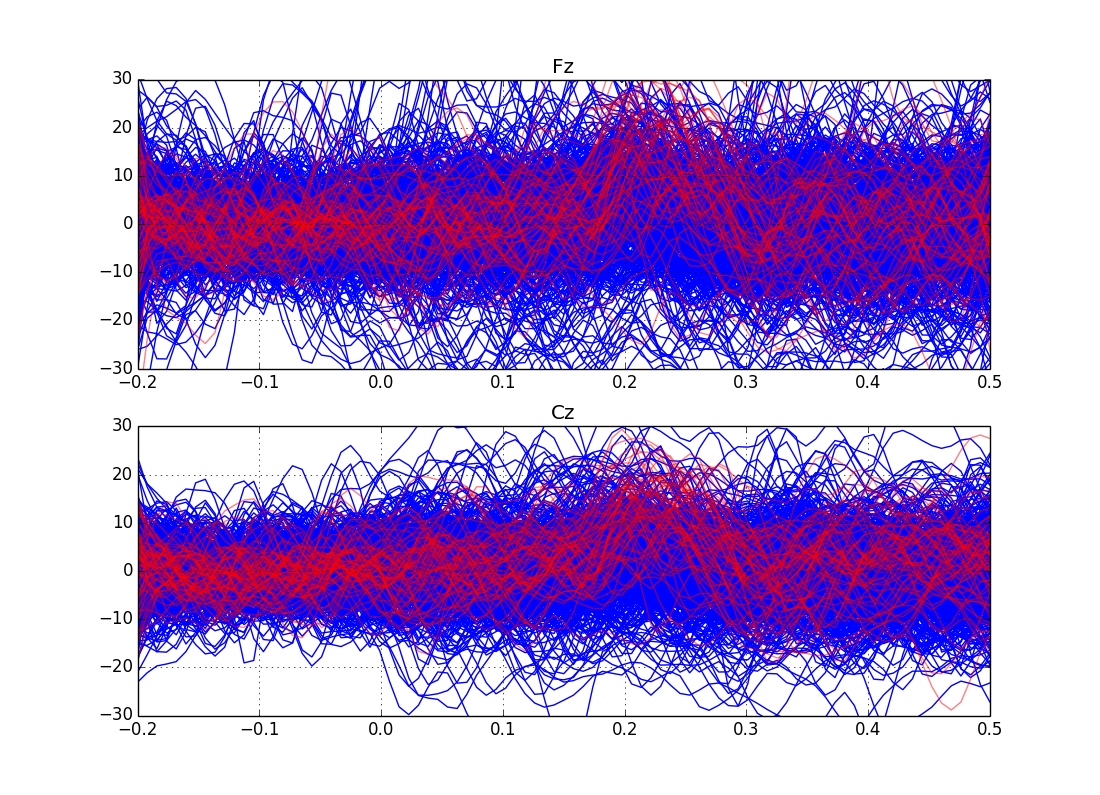
\includegraphics[scale=0.55, trim=10mm 15mm 10mm 15mm, clip=True]{pics/sygnal_toz.png}
\caption{Wykres sygnałów target (czerwony) i non-target (niebieski) dla dwóch najlepszych kanałów dla filtru tożsamościowego. Oś odciętych -- potencjał w  $\mu$V, oś rzędnych -- czas w s, zero oznacza wystąpienie bodźca.}
\label{sygnal_toz}
\end{figure}

\subsection{Transformata Hjorta}

Na rysunku \ref{macierz_hjorth} przedstawiono macierz uśrednionych sygnałów dla przebiegów target (czerwony) i non-target (niebieski). Dla transformaty Hjorta do analizy wybrano kanały T5 oraz Pz. Wszystkie przebiegi target i non-target dla tych kanałów przedstawiono na rysunku \ref{sygnal_hjorth}.

\begin{figure}
\centering
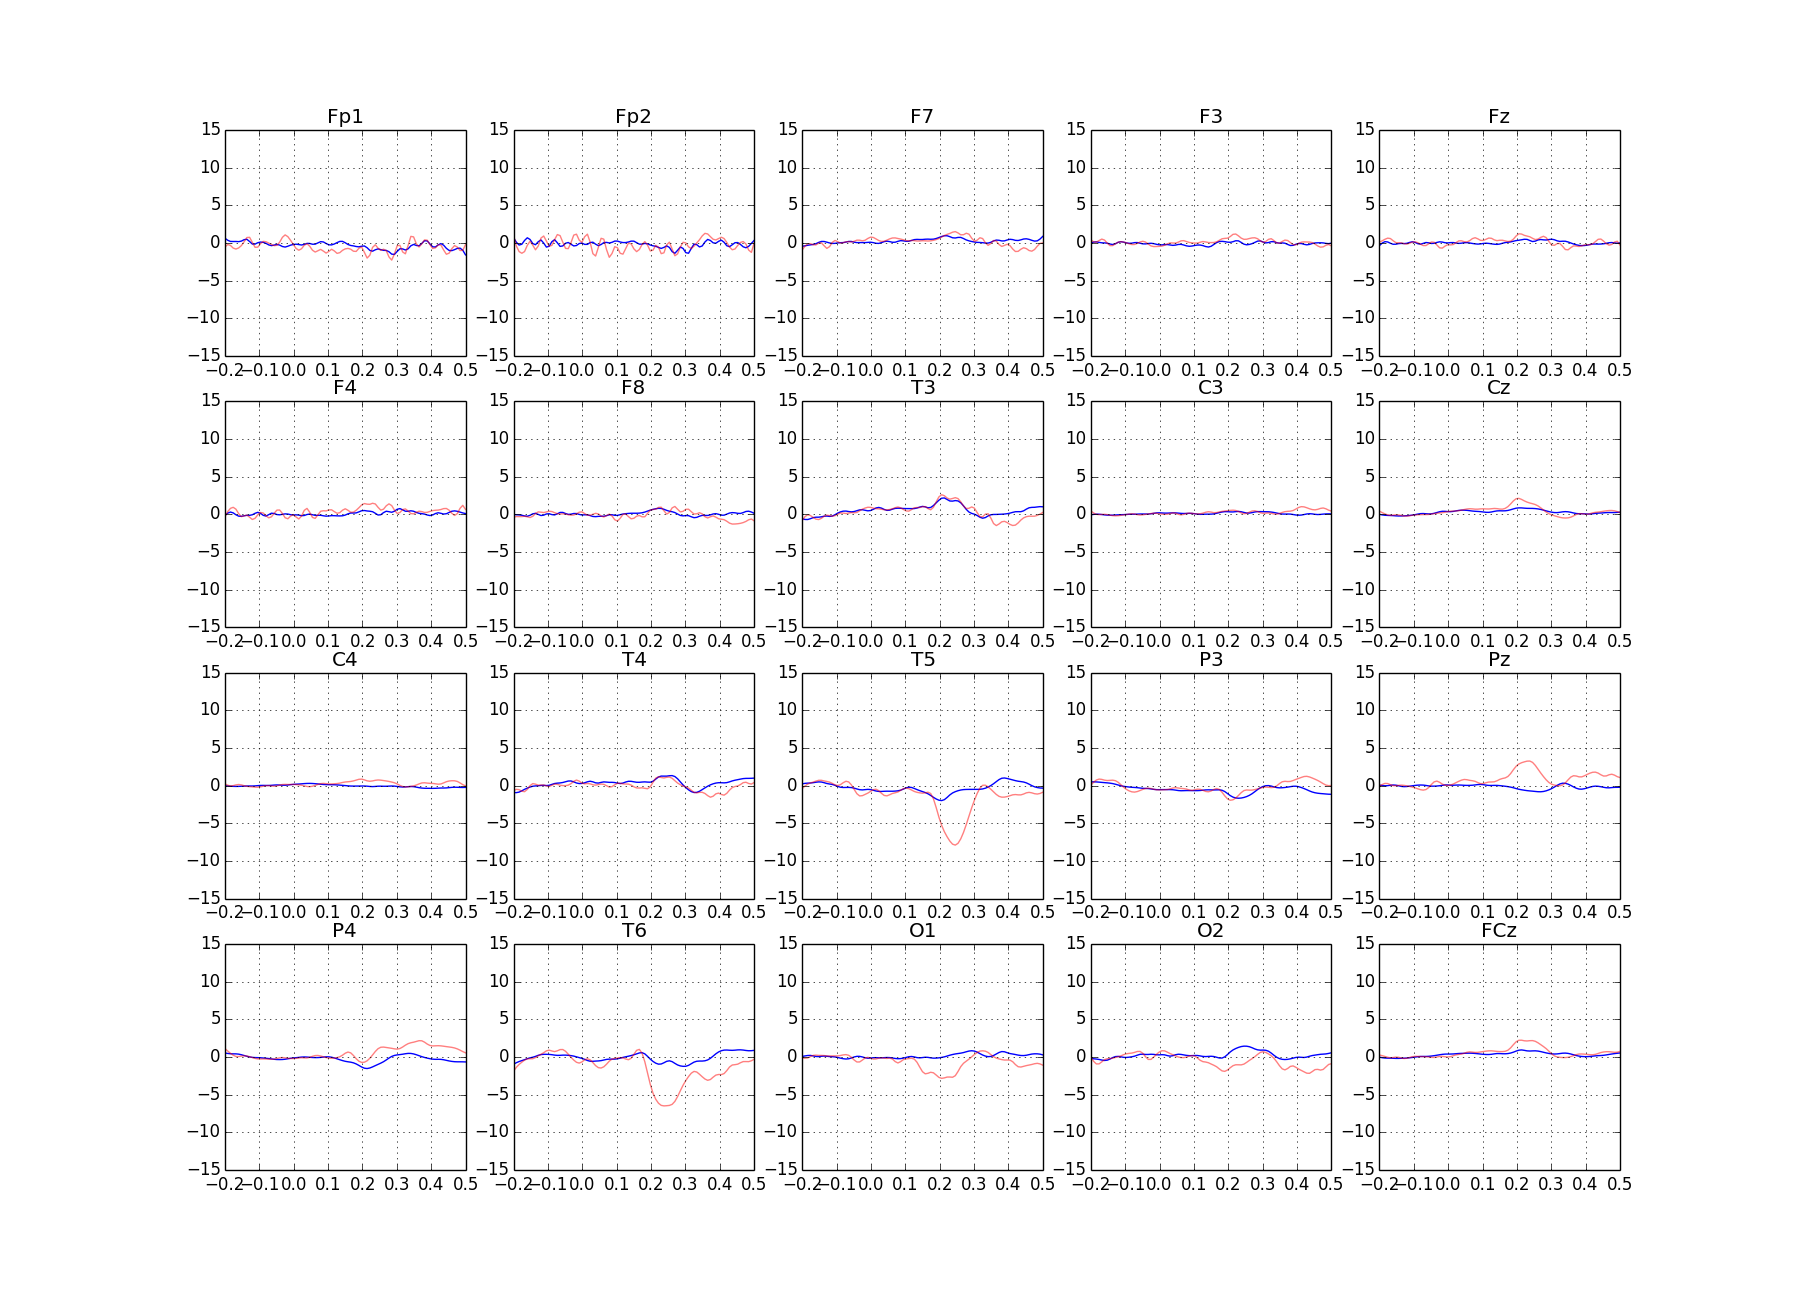
\includegraphics[scale=0.35, trim=10mm 25mm 10mm 25mm, clip=True]{pics/macierz_hjorth.png}
\caption{Macierz sygnałów uśrednionych target (czerwony) i non-target (niebieski) dla transformaty Hjorta. Oś odciętych -- potencjał w  $\mu$V, oś rzędnych -- czas w s, zero oznacza wystąpienie bodźca.}
\label{macierz_hjorth}
\end{figure}

\begin{figure}
\centering
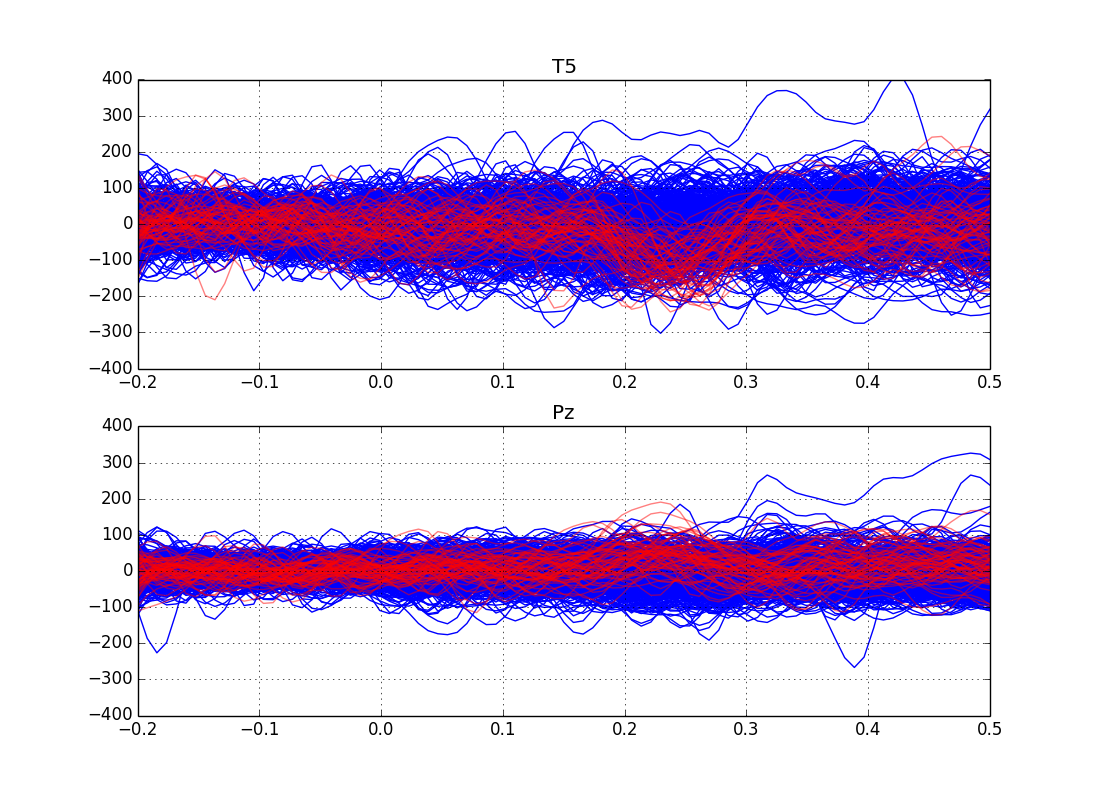
\includegraphics[scale=0.55, trim=10mm 15mm 10mm 15mm, clip=True]{pics/sygnal_hjorth.png}
\caption{Wykres sygnałów target (czerwony) i non-target (niebieski) dla dwóch najlepszych kanałów dla transformaty Hjorta. Oś odciętych -- potencjał w  $\mu$V, oś rzędnych -- czas w s, zero oznacza wystąpienie bodźca.}
\label{sygnal_hjorth}
\end{figure}

\subsection{Wspólny wzorzec przestrzenny}

Po zastosowaniu CSP dla macierzy kanałów ich pierwotne nazwy tracą swoje zastosowanie ze względu na przemnożenie każdego z nich przez macierz przejścia CSP. Kanały posegregowane są malejąco względem wartości cech rozróżniających przebiegi target od przebiegów non-target i przedstawiono je na rysunku \ref{macierz_csp}. Do analizy wybrano kanały 0 i 1, ich przebiegi zaprezentowano na rysunku \ref{sygnal_csp}.

\begin{figure}
\centering
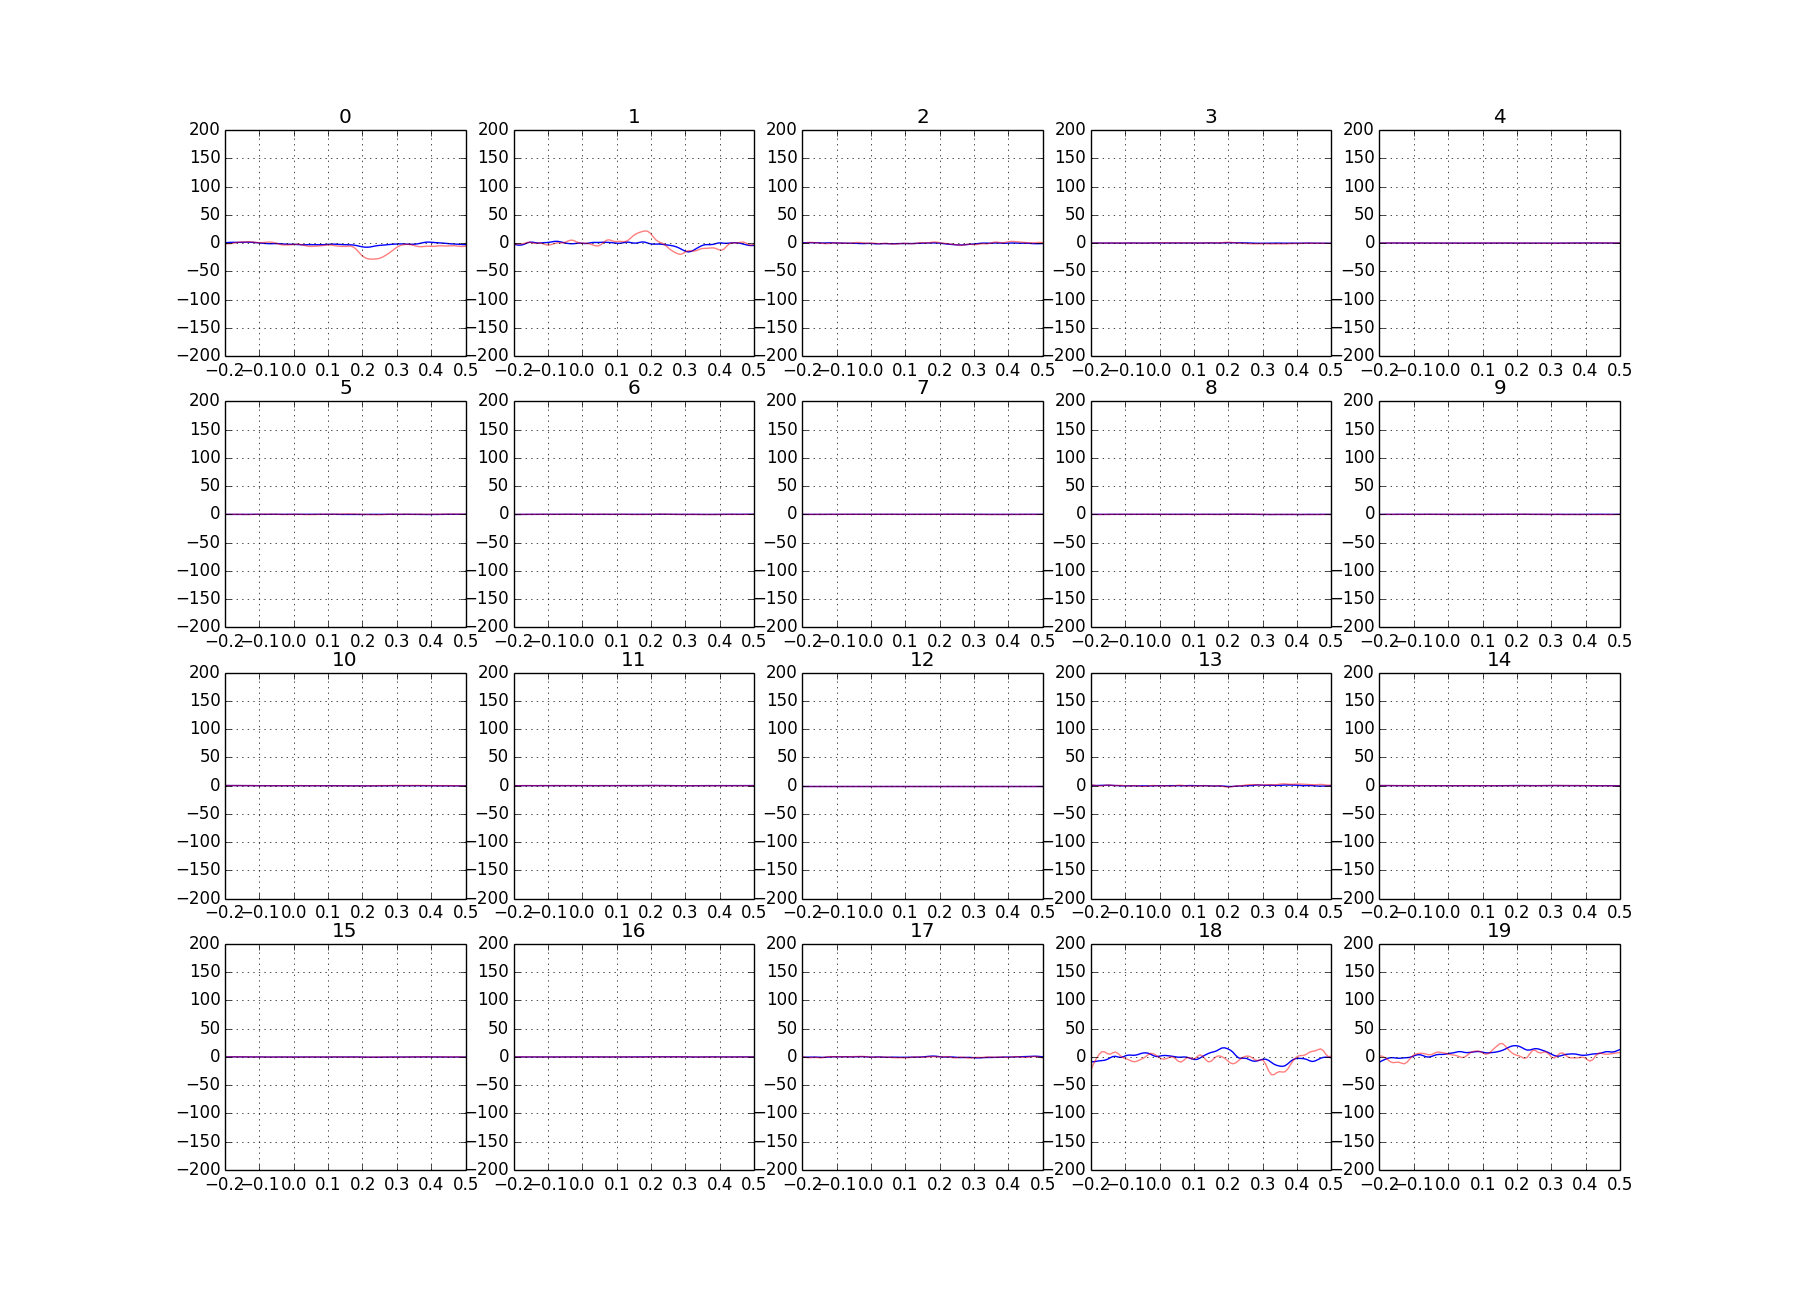
\includegraphics[scale=0.35, trim=10mm 25mm 10mm 25mm, clip=True]{pics/macierz_csp.png}
\caption{Macierz sygnałów uśrednionych target (czerwony) i non-target (niebieski) dla CSP. Oś odciętych -- potencjał w  $\mu$V, oś rzędnych -- czas w s, zero oznacza wystąpienie bodźca.}
\label{macierz_csp}
\end{figure}

\begin{figure}
\centering
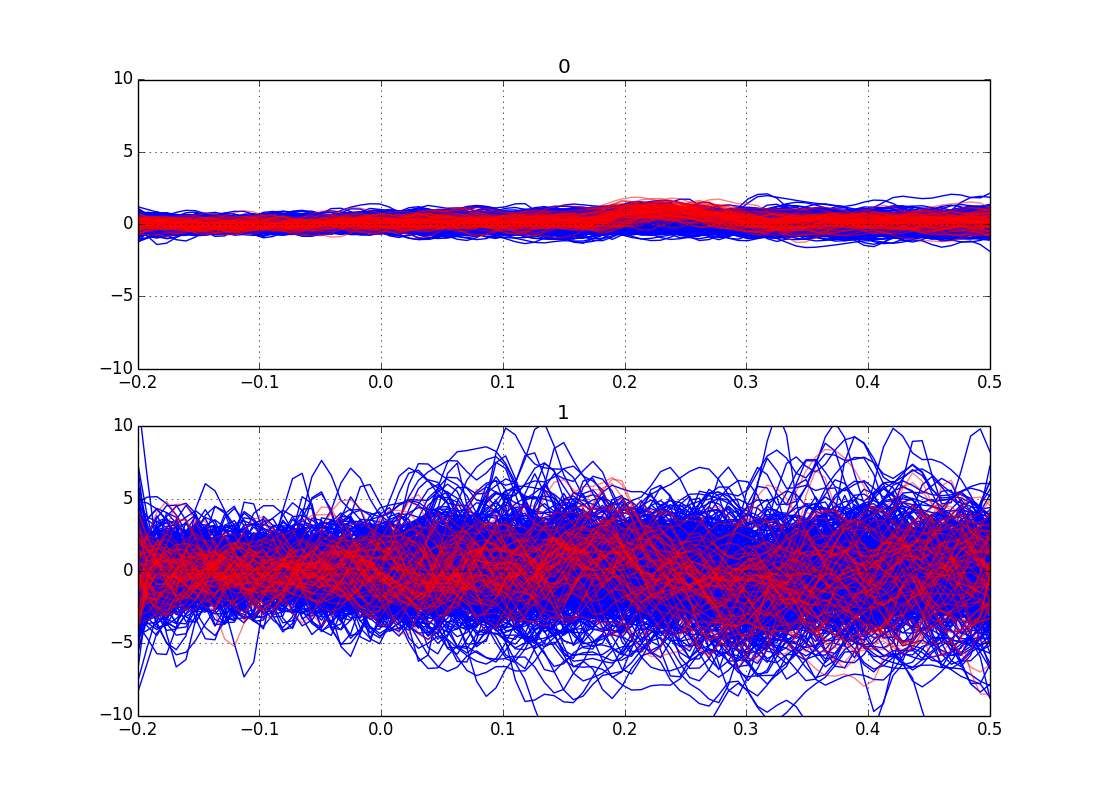
\includegraphics[scale=0.55, trim=10mm 15mm 10mm 15mm, clip=True]{pics/sygnal_csp.png}
\caption{Wykres sygnałów target (czerwony) i non-target (niebieski) dla dwóch najlepszych kanałów dla CSP. Oś odciętych -- potencjał w  $\mu$V, oś rzędnych -- czas w s, zero oznacza wystąpienie bodźca.}
\label{sygnal_csp}
\end{figure}


\FloatBarrier
\section{Porównanie cech}
\label{porownanie_cech}
Dla sygnałów zaprezentowanych w dziale \ref{sygnaly} obliczona została odległość Mahalanobisa (rozdział \ref{miara}). Ze względu na niewielką liczbę zarejestrowanych przebiegów dla każdego filtru przestrzennego zastosowano metodę bootstrap. Z obydwu grup (target i non-target) losowano po 10 przebiegów, które uśredniano ze sobą wykorzystując odpowiednio 2, 4, 10 z nich i porównywano z uśrednionymi pozostałymi realizacjami. Operację za każdym razem powtarzano 100 razy.

W rozdziałach \ref{roz_cecha_toz}, \ref{roz_cecha_hjorth} oraz \ref{roz_cecha_csp} zaprezentowano wyniki działania klasyfikatora dla sygnału, na którym zastosowano kolejno filtry przestrzenne omawiane w pracy.

\subsection{Filtr tożsamościowy}
\label{roz_cecha_toz}
Na rysunkach \ref{cecha_toz_2}, \ref{cecha_toz_4}, \ref{cecha_toz_10} zaprezentowano rozkład cech dla sygnałów target (niebieski) i sygnałów non-target (czerwony) dla odpowiednio dwóch, czterech i dziesięciu uśrednionych realizacji.

Zgodnie z oczekiwaniami separacja obydwu zbiorów rośnie wraz ze zwiększaniem się liczby uśrednionych realizacji. Niestety zarówno dla dwóch jak i czterech uśrednionych realizacji odległość pomiędzy zbiorami target i non-target jest niewielka względem rozrzutu tych zbiorów co przy zastosowaniu tego algorytmu w urządzeniu BCI prowadziłoby do błędnej interpretacji decyzji użytkownika.


%nie jest możliwe jednoznaczne oddzielenie zbiorów co przy zastosowaniu tego algorytmu w urządzeniu BCI prowadziłoby do błędnej interpretacji decyzji użytkownika.

\begin{figure}
\centering
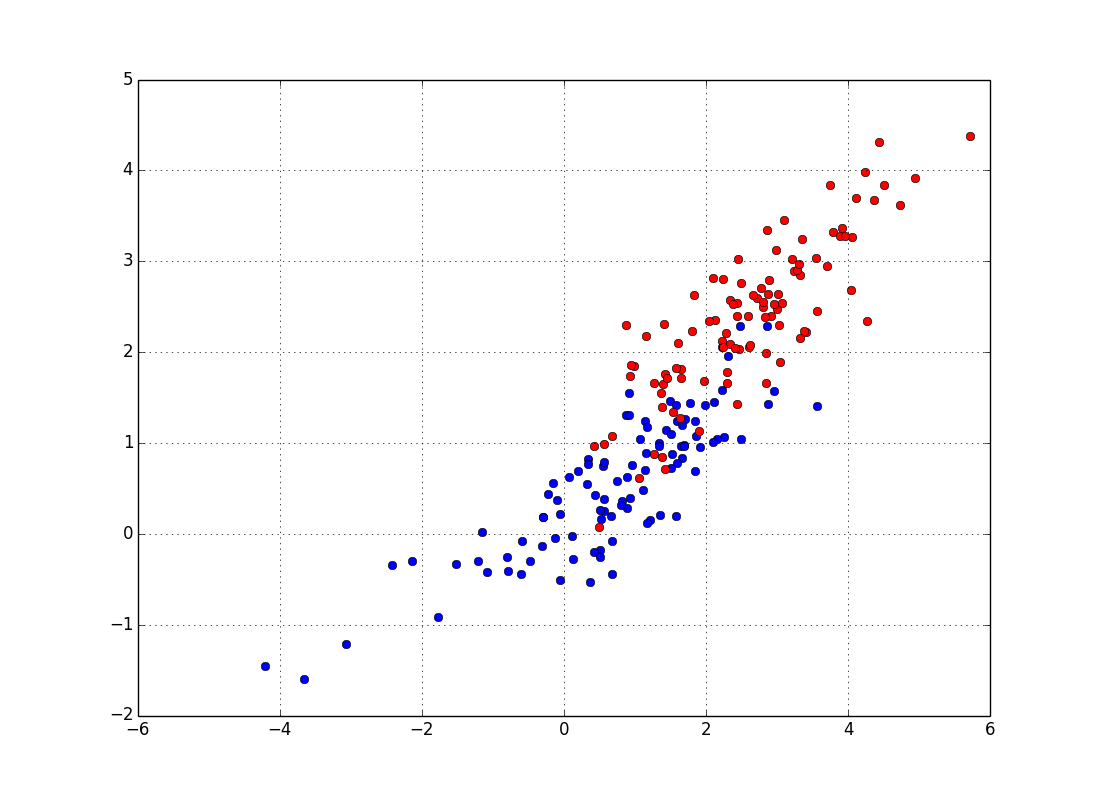
\includegraphics[scale=0.55, trim=10mm 15mm 10mm 18mm, clip=True]{pics/cecha_toz_2.png}
\caption{Rozkład cech dla dwóch najlepszych kanałów dla sygnałów target (czerwony) i non-target (niebieski) przy dwóch uśrednionych realizacjach dla filtru tożsamościowego. Na osiach wartość funkcji korelacji.}
\label{cecha_toz_2}
\end{figure}

\begin{figure}
\centering
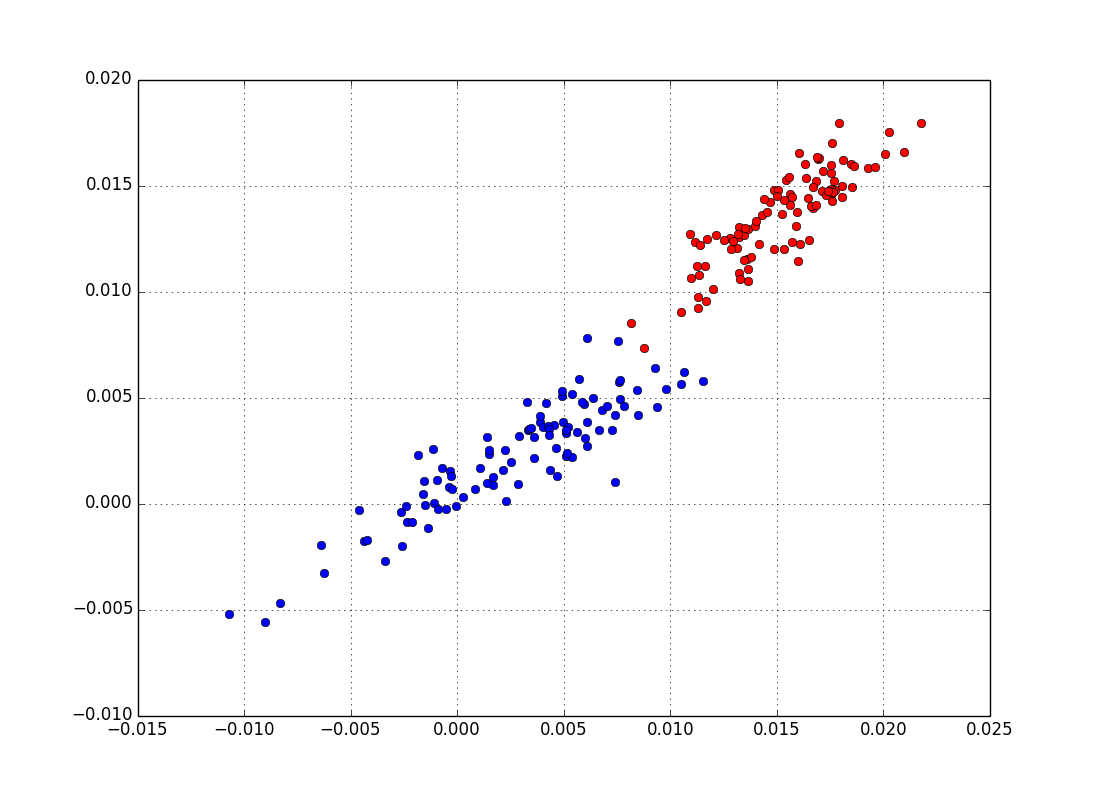
\includegraphics[scale=0.55, trim=10mm 15mm 10mm 18mm, clip=True]{pics/cecha_toz_4.png}
\caption{Rozkład cech dla dwóch najlepszych kanałów dla sygnałów target (czerwony) i non-target (niebieski) przy czterech uśrednionych realizacjach dla filtru tożsamościowego. Na osiach wartość funkcji korelacji.}
\label{cecha_toz_4}
\end{figure}

\begin{figure}
\centering
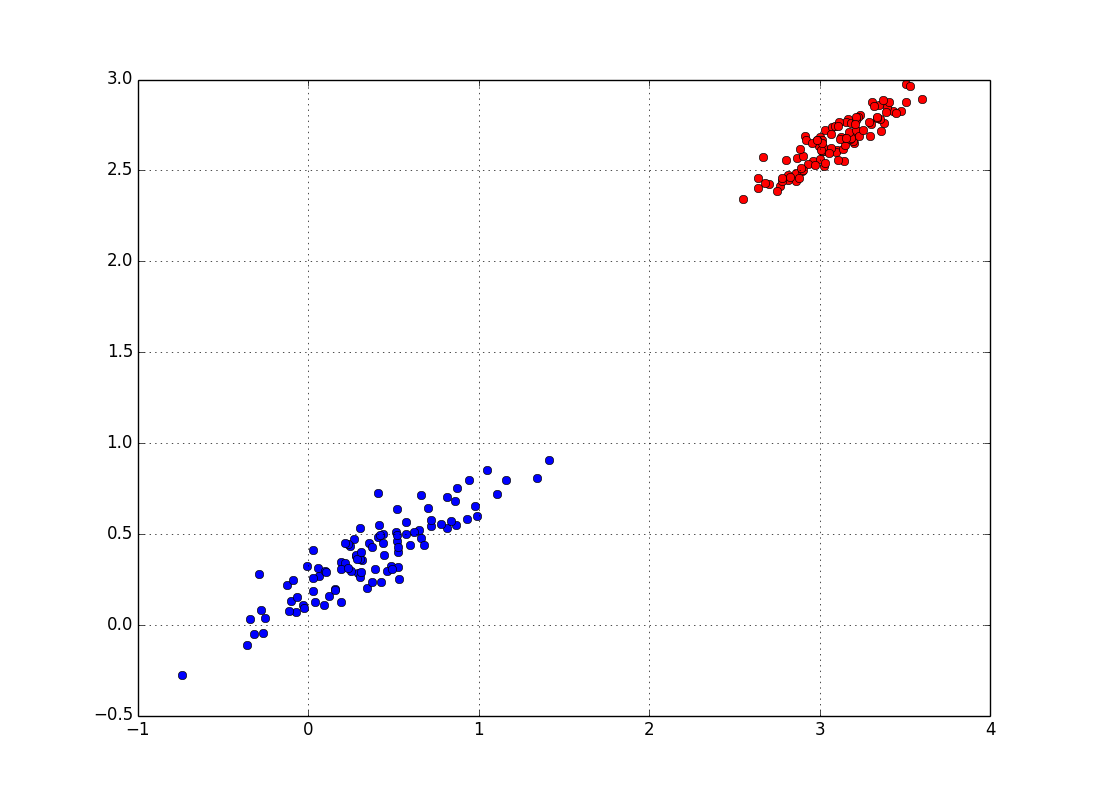
\includegraphics[scale=0.55, trim=10mm 15mm 10mm 18mm, clip=True]{pics/cecha_toz_10.png}
\caption{Rozkład cech dla dwóch najlepszych kanałów dla sygnałów target (czerwony) i non-target (niebieski) przy dziesięciu uśrednionych realizacjach dla filtru tożsamościowego. Na osiach wartość funkcji korelacji.}
\label{cecha_toz_10}
\end{figure}

\subsection{Transformata Hjorta}
\label{roz_cecha_hjorth}
Podobnie jak w rodziale \ref{roz_cecha_toz} na rysunkach \ref{cecha_hjorth_2}, \ref{cecha_hjorth_4}, \ref{cecha_hjorth_10} przedstawiony został rozkład cech dla sygnałów target (niebieski) i sygnałów non-target (czerwony) dla odpowiednio dwóch, czterech i dziesięciu uśrednionych realizacji przy zastosowaniu transformaty Hjorta. W tym przypadku w odróżnieniu od filtru tożsamościowego już przy czterech uśrednionych realizacjach zachodzi bardzo dobra separacja zbiorów sygnałów target i non-target względem ich rozrzutu wykluczająca błędną interpretację decyzji w urządzeniu BCI.

\begin{figure}
\centering
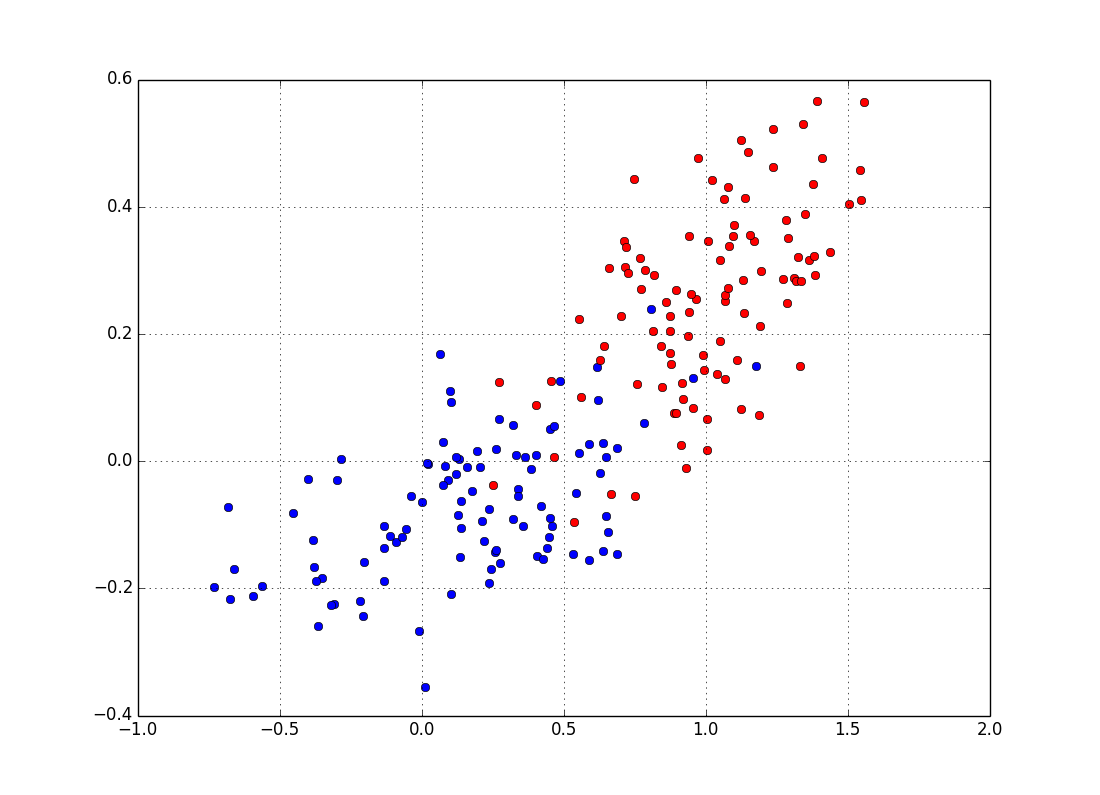
\includegraphics[scale=0.55, trim=10mm 15mm 10mm 18mm, clip=True]{pics/cecha_hjorth_2.png}
\caption{Rozkład cech dla dwóch najlepszych kanałów dla sygnałów target (czerwony) i non-target (niebieski) przy dwóch uśrednionych realizacjach dla transformaty Hjorta. Na osiach wartość funkcji korelacji.}
\label{cecha_hjorth_2}
\end{figure}

\begin{figure}
\centering
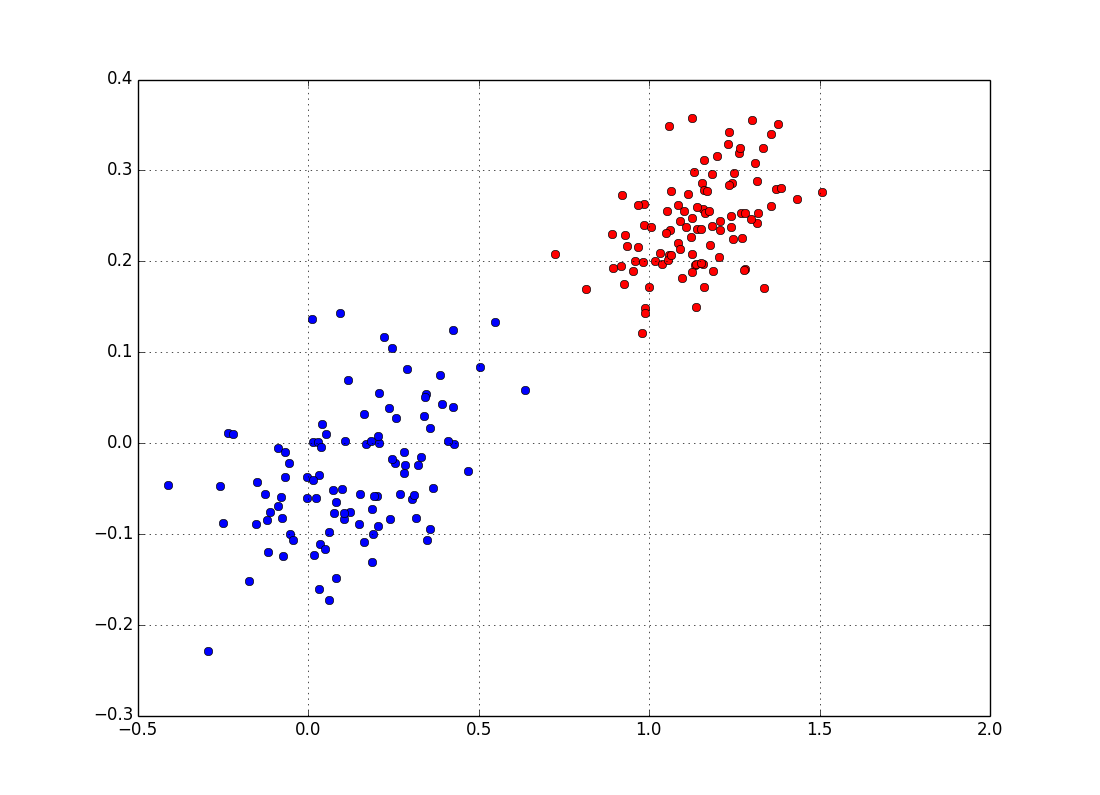
\includegraphics[scale=0.55, trim=10mm 15mm 10mm 18mm, clip=True]{pics/cecha_hjorth_4.png}
\caption{Rozkład cech dla dwóch najlepszych kanałów dla sygnałów target (czerwony) i non-target (niebieski) przy czterech uśrednionych realizacjach dla transformaty Hjorta. Na osiach wartość funkcji korelacji.}
\label{cecha_hjorth_4}
\end{figure}

\begin{figure}
\centering
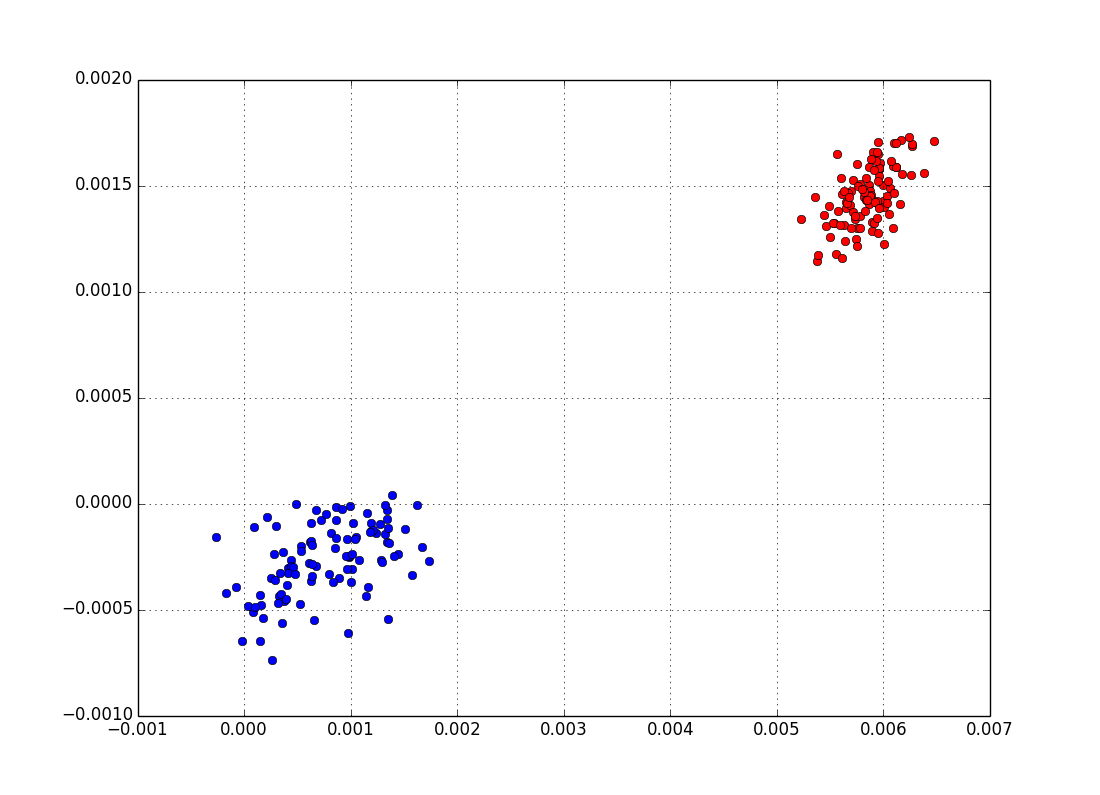
\includegraphics[scale=0.55, trim=10mm 15mm 10mm 18mm, clip=True]{pics/cecha_hjorth_10.png}
\caption{Rozkład cech dla dwóch najlepszych kanałów dla sygnałów target (czerwony) i non-target (niebieski) przy dziesięciu uśrednionych realizacjach dla transformaty Hjorta. Na osiach wartość funkcji korelacji.}
\label{cecha_hjorth_10}
\end{figure}

\subsection{Wspólny wzorzec przestrzenny}
\label{roz_cecha_csp}
W przypadku CSP na rysunku \ref{cecha_csp_2} widać, że już przy dwóch uśrednionych przebiegach następuje praktycznie całkowite rozseparowanie zbiorów sygnałów target i non-target. Ponadto dla czterech i dziesięciu uśrednionych realizacji (rys. \ref{cecha_csp_4}, \ref{cecha_csp_10}) separacja zbiorów jest zdecydowanie lepsza niż dla poprzednich filtrów przestrzennych zaprezentowanych w rozdziałach \ref{roz_cecha_toz} i \ref{roz_cecha_hjorth}.

\begin{figure}
\centering
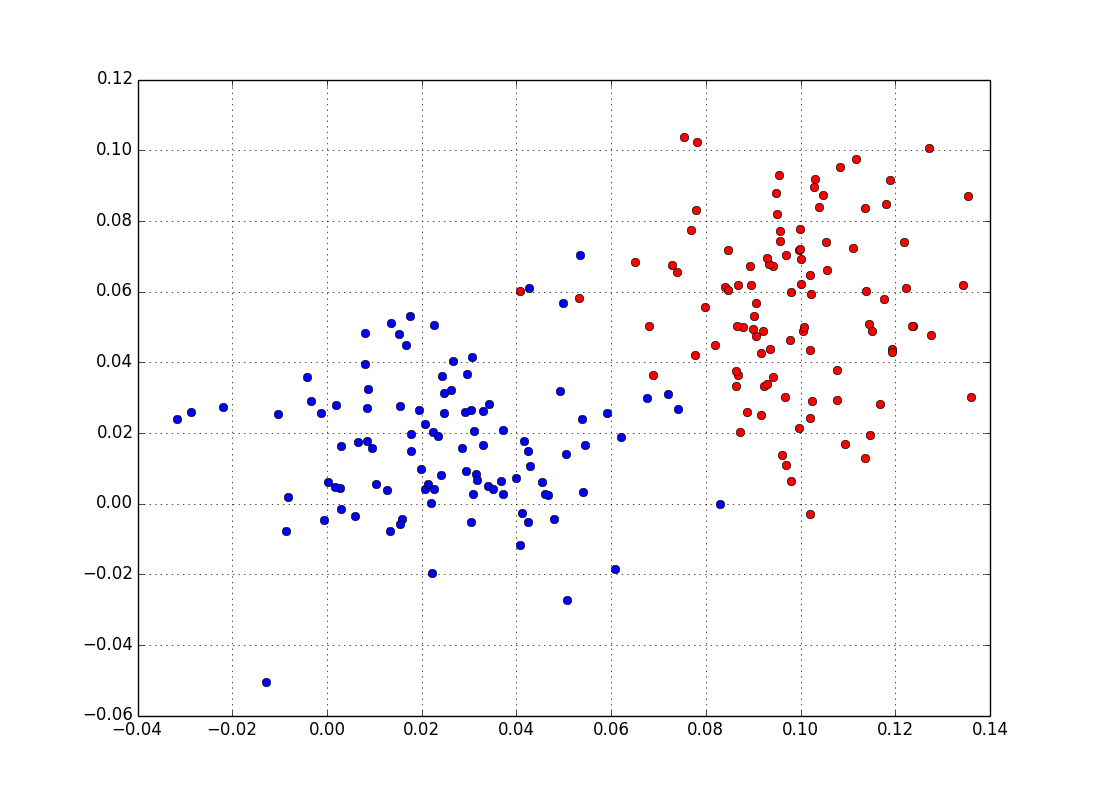
\includegraphics[scale=0.55, trim=10mm 15mm 10mm 18mm, clip=True]{pics/cecha_csp_2.png}
\caption{Rozkład cech dla dwóch najlepszych kanałów dla sygnałów target (czerwony) i non-target (niebieski) przy dwóch uśrednionych realizacjach dla CSP. Na osiach wartość funkcji korelacji.}
\label{cecha_csp_2}
\end{figure}

\begin{figure}
\centering
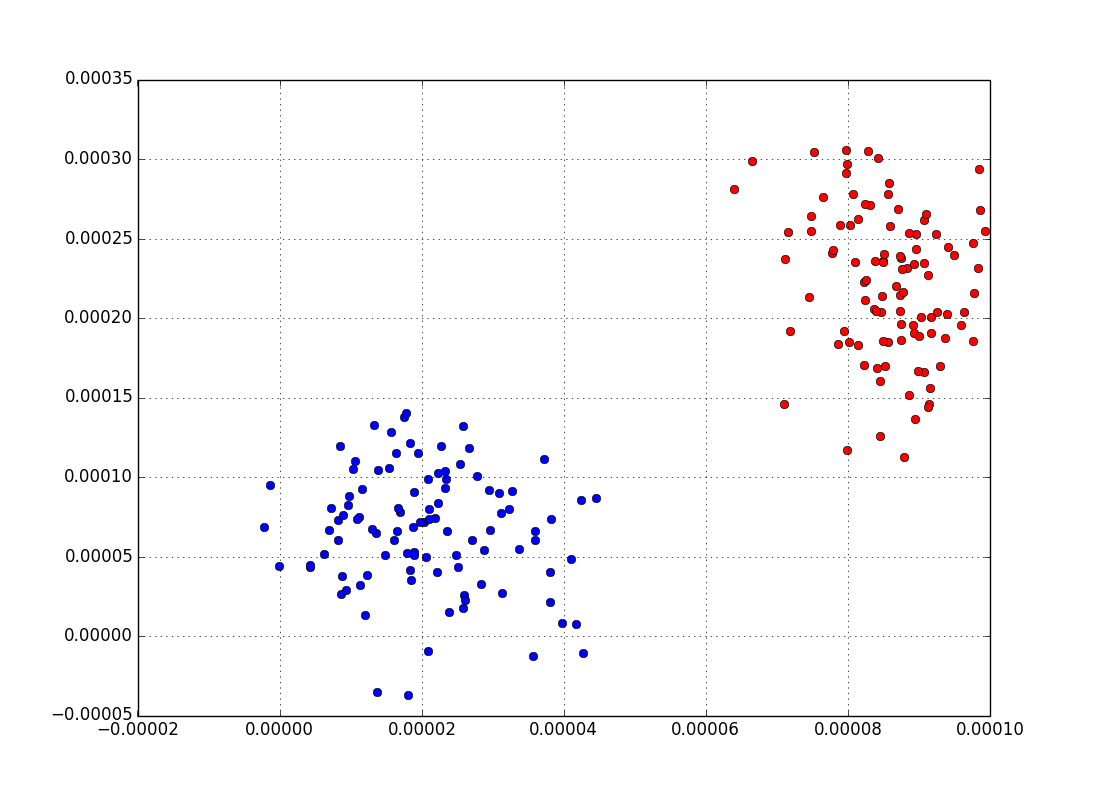
\includegraphics[scale=0.55, trim=10mm 15mm 10mm 18mm, clip=True]{pics/cecha_csp_4.png}
\caption{Rozkład cech dla dwóch najlepszych kanałów dla sygnałów target (czerwony) i non-target (niebieski) przy czterech uśrednionych realizacjach dla CSP. Na osiach wartość funkcji korelacji.}
\label{cecha_csp_4}
\end{figure}

\begin{figure}
\centering
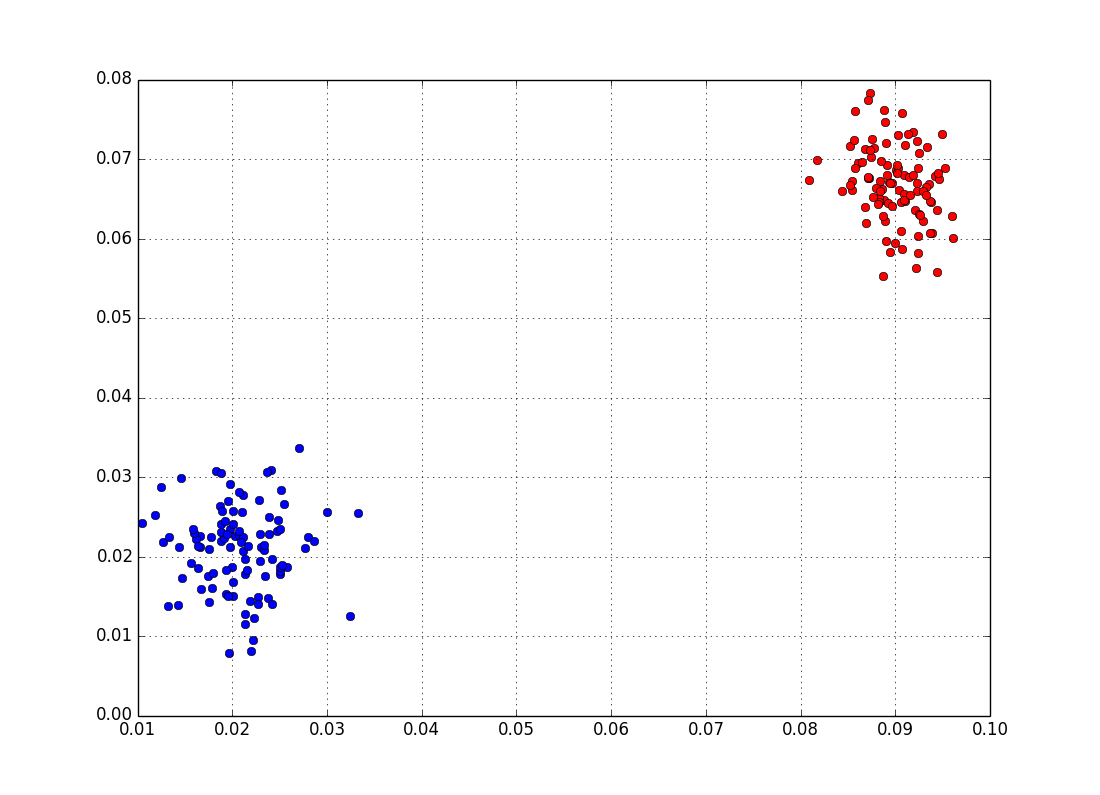
\includegraphics[scale=0.55, trim=10mm 15mm 10mm 18mm, clip=True]{pics/cecha_csp_10.png}
\caption{Rozkład cech dla dwóch najlepszych kanałów dla sygnałów target (czerwony) i non-target (niebieski) przy dziesięciu uśrednionych realizacjach dla CSP. Na osiach wartość funkcji korelacji.}
\label{cecha_csp_10}
\end{figure}

\FloatBarrier
\section{Odległość Mahalanobisa}
Na rysunku \ref{mahalanobis_pic} przedstawiono zależność odległości Mahalanobisa od liczby uśrednionych realizacji dla wszystkich rodzajów omawianych filtrów przestrzennych. Zgodnie z oczekiwaniami oraz widocznymi zależnościami przedstawionymi na wykresach w rozdziale \ref{porownanie_cech} widać, że najlepsze rezultaty osiągnięto dla CSP, gorsze dla transformaty Hjorta, a najgorsze dla filtru tożsamościowego. 

\begin{figure}
\centering
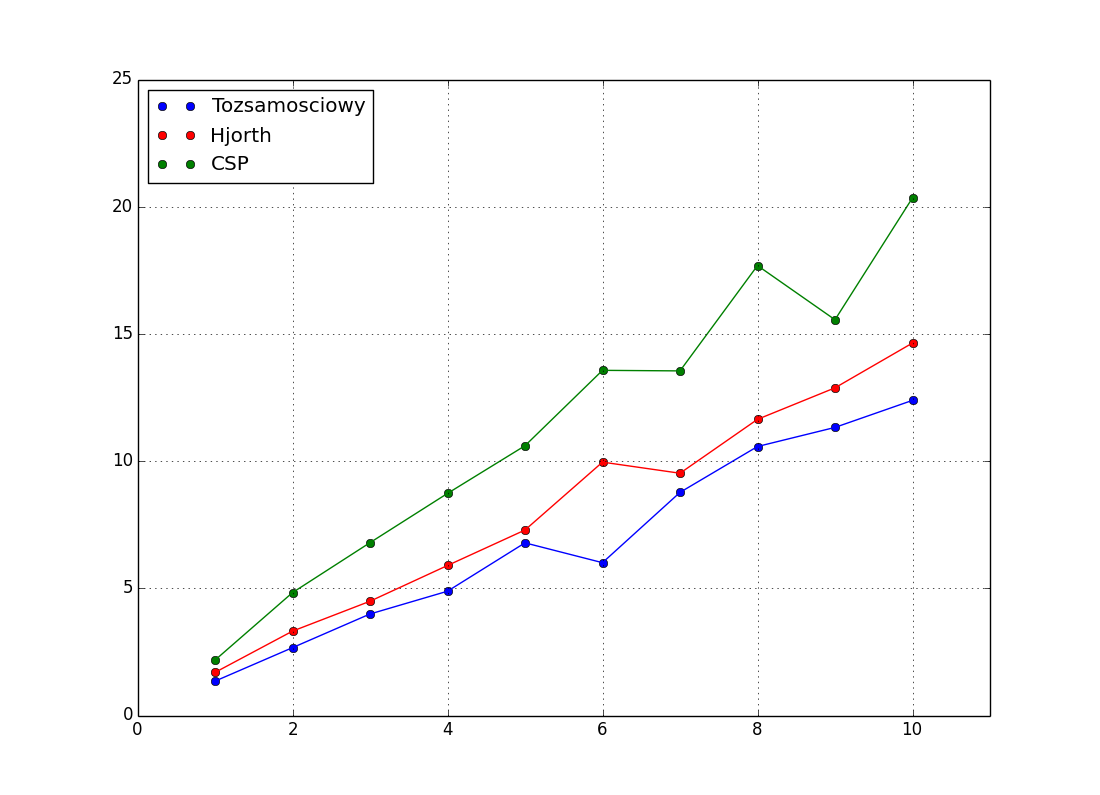
\includegraphics[scale=0.6, trim=10mm 15mm 10mm 18mm, clip=True]{pics/mahalanobis.png}
\caption{Zależność odległości Mahalanobisa od liczby uśrednianych realizacji dla każdego prezentowanego filtru. Na osi rzędnych odległość Mahalanobisa, na osi odciętych liczba uśrednionych realizacji.}
\label{mahalanobis_pic}
\end{figure}

\chapter{Dyskusja i Wnioski}
Filtry przestrzenne są obecnie szeroko stosowane w detekcji potencjałów wywołanych oraz wyobrażeń ruchowych w oprogramowaniu BCI takich jak OpenBCI \citep{obci_conf}, OpenVibe \citep{renard2010}. Ze względu na wymaganą kalibrację oraz złożoność obliczeniową procesu wyznaczania macierzy przejścia nie jest możliwe zastosowanie CSP w każdym paradygmacie BCI.

Z przedstawionych rezultatów jasno wynika, że zastosowanie filtrów przestrzennych znacząco poprawia wykrywalność wzrokowego potencjału P300 w sygnale EEG. Możliwość zastosowania CSP w praktyce potwierdziła wystawa Mózg 2013, na której prezentowane urządzenie BCI zostało przetestowane przez około trzystu zwiedzających z bardzo dobrymi rezultatami. W wykrywaniu potencjału P300 oraz SSVEP wykorzystano filtr CSP w identycznej postaci jak przedstawiony w tej pracy.

\bibliography{biblio}
\end{document}
